\begin{figure}

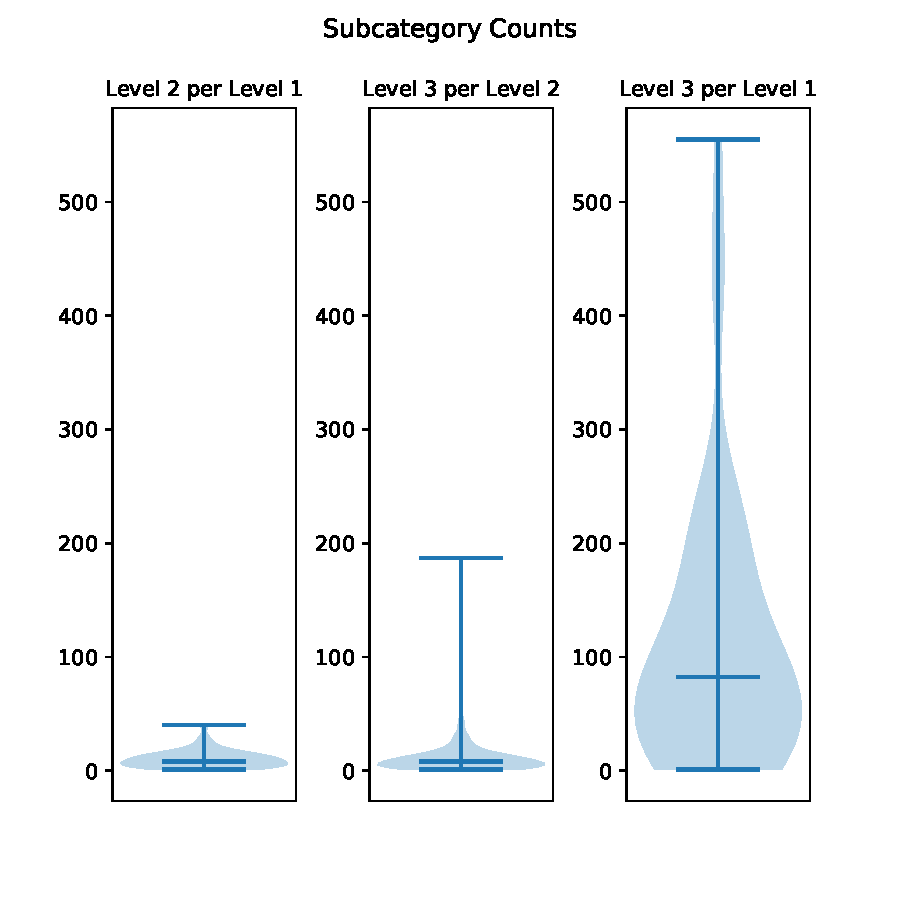
\includegraphics[width=\columnwidth]{img/catcount}
\caption{
This violin plot compares hierarchical category branching in the Cdiscount dataset.
The leftmost subplot presents the distribution of the number of second level subcategories in each top-level category.
The middle subplot presents the distribution of the number of third (bottom) level subcategories in each second level category.
The rightmost subplot presents the distribution of the number of bottom level subcategories in each first level category.
Going from first to second level and second to third level, categories branch by a median factor of approximately 10. 
From first to third level, categories branch by a median factor of approximately 100.
All three branching factor distributions have long right tails.
For example, going from second to third level, some categories are observed to branch by a factor of more than 150.
In all three subplots, horizontal bars mark the 0, 50, and 100th percentile counts.
}
\label{fig:catcount}

\end{figure}